\section{Constructing the queuing model}\label{sec:wasserstein}

The simplest queuing model using the data available is an \(M|M|c\) queue with
multiple classes. In this model, the following assumptions are made:
\begin{enumerate}
    \item Inter-arrival and service times of patients are each exponential with
        some mean.
    \item There are $c$ servers available to arriving patients at a single node
        representing the overall resource availability at the hospital.
    \item There is no queue or system capacity.
    \item A first-in first-out service policy is implemented.
\end{enumerate}

Each group of patients has its own arrival distribution. The parameter of this
distribution is taken to be the reciprocal of the mean inter-arrival times for
that group.

Like arrivals, each group of patients has its own service time distribution.
The parameter of this distribution is approximated via the length of a patient's
stay, i.e.\ the total time spent in the system. Without full details of the
process order or idle periods during a spell, some assumption must be made about
the true `service' time in relation to the time spent in hospital. This work
considers the mean service time, \(\frac{1}{\mu}\), to be directly proportional
to the mean total system time, \(\frac{1}{\phi}\), such that:
\begin{equation}
    \mu = p \phi
\end{equation}

\noindent where \(p \in \interval[open left]{0}{1}\) is some parameter to be
determined for each group, denoted by \(p_i\) for group \(i\).

As the full details of how the patients move through the hospital system, and
the details of the system itself, are unknown, an appropriate number of servers
\(c\) must be found as well as each \(p_i\).

In order to evaluate appropriate values of each \(p_i\) and the value of \(c\),
the system is simulated across of parameter space. Then, for each set of
parameters, the total time distribution is compared with that in the available
data via the (first) Wasserstein distance. This distance measures the
approximate `minimal work' required to move between two probability
distributions where `work' can be loosely defined as the product of how much of
the distribution's mass must be to be moved with the distance it must be moved
by. More formally, the Wasserstein distance between two probability
distributions \(U\) and \(V\) is defined as:
\begin{equation}\label{eq:wasserstein}
    W(U, V) = \int_{0}^{1} \left\vert F^{-1}(t) - G^{-1}(t) \right\vert dt
\end{equation}

\noindent where \(F\) and \(G\) are the cumulative density functions of \(U\)
and \(V\) respectively. A proof of~\eqref{eq:wasserstein} is presented
in~\cite{RTC17}. The parameter set with the smallest maximum distance over a
number of runs is then taken to be the most appropriate.

\begin{figure}
    \centering%
    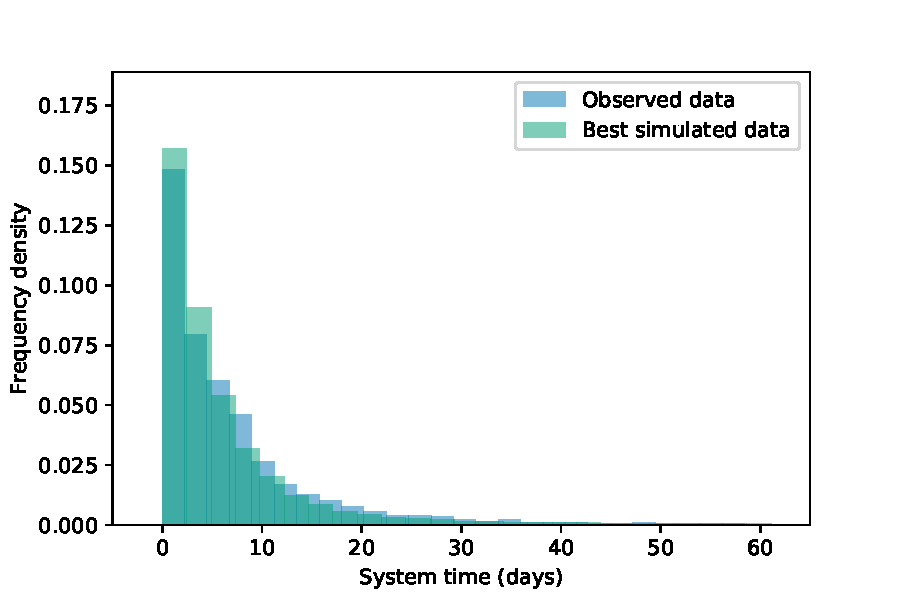
\includegraphics[width=\imgwidth]{best_params}
    \caption{A histogram of the simulated and observed length of stay data for
             the best parameter set.}\label{fig:best_params}
\end{figure}

\begin{figure}
    \centering%
    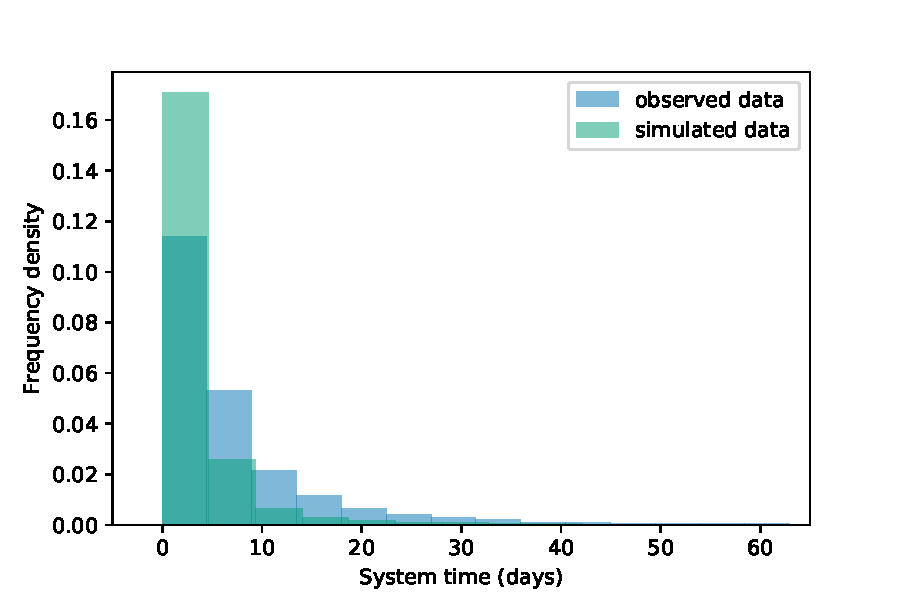
\includegraphics[width=\imgwidth]{worst_params}
    \caption{A histogram of the simulated and observed length of stay data for
             the worst parameter set.}\label{fig:worst_params}
\end{figure}

The results of this parameter estimation can be summarised in
Figures~\ref{fig:best_params}~and~\ref{fig:worst_params}. Each figure shows a
comparison between the observed lengths of stay across all groups with the newly
simulated data with the best and worst parameter sets respectively. Indeed, it
can be seen that, in the best case, a very close fit has been found. Meanwhile,
Figure~\ref{fig:worst_params} highlights the importance of good parameter
estimation under this model since the likelihood of short-stay patient arrivals
has been inflated disproportionately.
